\documentclass[modern]{aastex61}

% All the packages
%\usepackage[letterpaper]{geometry}
\usepackage{microtype}
\usepackage{url}
\usepackage{amsmath}
\usepackage{mathtools}
\usepackage{esint}
\usepackage{amssymb}
\usepackage{natbib}
\usepackage{multirow}
\usepackage{graphicx}
\usepackage{scalerel}
\usepackage{calc}
\usepackage{etoolbox}
\usepackage{marginnote}
\usepackage{nicefrac}
\usepackage{tabstackengine}
\usepackage{diagbox}
\usepackage[makeroom]{cancel}
\usepackage{mathdots}
\usepackage{bbm}
\usepackage{booktabs}
\usepackage{xspace}
\stackMath

% Bibliography stuff
\bibliographystyle{aasjournal}

% Shorthand for this paper
\newcommand{\starry}{\textsf{starry}\xspace}

% References to text content
\newcommand{\documentname}{\textsl{article}}
\newcommand{\figureref}[1]{\ref{fig:#1}}
\newcommand{\Figure}[1]{Figure~\figureref{#1}}
\newcommand{\figurelabel}[1]{\label{fig:#1}}
\renewcommand{\eqref}[1]{\ref{eq:#1}}
\newcommand{\Eq}[1]{Equation~(\eqref{#1})}
\newcommand{\eq}[1]{\Eq{#1}}
\newcommand{\eqalt}[1]{Equation~\eqref{#1}}
\newcommand{\eqlabel}[1]{\label{eq:#1}}

% Add script hyperlinks as margin notes
\definecolor{proofcolor}{rgb}{0.1216,0.4667,0.7059}
\newcommand{\python}[1]{\marginnote{\href{https://github.com/rodluger/starry/tree/master/tex/figures/#1.py}{
\includegraphics[width=0.9cm]{figures/python.png}}}}
\newcommand{\mathematica}[1]{\marginnote{\href{https://github.com/rodluger/starry/tree/master/tex/notebooks/#1.nb}{
\includegraphics[width=0.6cm]{figures/mathematica.png}}}}
\newcommand{\todoproof}{\marginnote{\href{}{
\includegraphics[width=0.4cm]{figures/todo.png}}}}
\newcommand{\todo}[2]{\marginnote{\color{red}\textbf{#1:}\\\scriptsize\textbf{#2}}}

% Force margin notes to always be on the right side
% https://tex.stackexchange.com/a/69624

% Math stuff
\newcommand{\ii}{\ensuremath{\mathbf{i}}}
\newcommand{\T}{\ensuremath{\mathrm{T}}}
\newcommand{\dd}{\ensuremath{ \mathrm{d}}}
\newcommand{\unit}[1]{{\ensuremath{\mathrm{#1}}}}
\newcommand{\bvec}[1]{{\ensuremath{\mathbf{#1}}}}
\newcommand{\avec}[1]{{\ensuremath{\vec{\mathbf{#1}}}}}
\newcommand{\x}{\ensuremath{\mbox{$x$}}}
\newcommand{\y}{\ensuremath{\mbox{$y$}}}
\newcommand{\z}{\ensuremath{\mbox{$z$}}}
\newcommand{\xhat}{\ensuremath{\mathbf{\hat{x}}}}
\newcommand{\yhat}{\ensuremath{\mathbf{\hat{y}}}}
\newcommand{\zhat}{\ensuremath{\mathbf{\hat{z}}}}
\DeclareMathAlphabet\mathbfcal{OMS}{cmsy}{b}{n}
\DeclareMathOperator{\Tr}{Tr}
\DeclarePairedDelimiter\ceil{\lceil}{\rceil}
\DeclarePairedDelimiter\floor{\lfloor}{\rfloor}
\definecolor{dim}{rgb}{0.8,0.8,0.8}
\newcolumntype{L}[1]{>{\raggedright\let\newline\\\arraybackslash\hspace{0pt}}m{#1}}
\setcounter{MaxMatrixCols}{20}
\newcommand{\sinphi}{\ensuremath{\mbox{$u$}}}
\newcommand{\sinlambda}{\ensuremath{\mbox{$v$}}}
\newcommand{\bigdot}{\scaleto{\cdot}{6pt}}

% Bases
\newcommand{\pbasis}{\ensuremath{\bvec{\tilde{p}}}}
\newcommand{\gbasis}{\ensuremath{\bvec{\tilde{g}}}}
\newcommand{\ybasis}{\ensuremath{\bvec{\tilde{y}}}}
\newcommand{\pbasisn}{\ensuremath{\tilde{p}_n}}
\newcommand{\gbasisn}{\ensuremath{\tilde{g}_n}}
\newcommand{\ybasisn}{\ensuremath{\tilde{y}_n}}
\newcommand{\AOne}{\ensuremath{\bvec{A_1}}}
\newcommand{\ATwo}{\ensuremath{\bvec{A_2}}}

% Code examples
\usepackage{listings}
\definecolor{codegreen}{rgb}{0,0.6,0}
\definecolor{codegray}{rgb}{0.5,0.5,0.5}
\definecolor{codepurple}{rgb}{0.58,0,0.82}
\definecolor{backcolour}{rgb}{0.95,0.95,0.95}
\lstdefinestyle{mystyle}{
    backgroundcolor=\color{backcolour},
    commentstyle=\color{codegreen},
    keywordstyle=\color{magenta},
    numberstyle=\tiny\color{codegray},
    stringstyle=\color{codepurple},
    basicstyle=\small\ttfamily,
    breakatwhitespace=false,
    breaklines=true,
    captionpos=b,
    keepspaces=true,
    numbers=left,
    numbersep=5pt,
    showspaces=false,
    showstringspaces=false,
    showtabs=false,
    tabsize=2,
    aboveskip=1em,
    belowskip=1em
}
\lstset{style=mystyle}

% Inverse diagonal dots
\makeatletter
\def\Ddots{\mathinner{\mkern1mu\raise\p@
\vbox{\kern7\p@\hbox{.}}\mkern2mu
\raise4\p@\hbox{.}\mkern2mu\raise7\p@\hbox{.}\mkern1mu}}
\makeatother

% Typography obsessions
\setlength{\parindent}{3.0ex}
\renewcommand\quad{\hskip\fontdimen3\font}


\begin{document}\raggedbottom\sloppy\sloppypar\frenchspacing

\setlength{\abovedisplayskip}{1.5em}
\setlength{\belowdisplayskip}{1.5em}

\title{%
    \textbf{STARRY}: Analytic Occultation Light Curves
}

\author[0000-0002-0296-3826]{Rodrigo Luger}
\affil{Department~of~Astronomy, University~of~Washington, Seattle, WA}
\author{others}

\keywords{methods: analytical --- techniques: photometric}

\begin{abstract}
    We derive analytical, closed form solutions for the total flux
    emitted or reflected from a celestial body in the direction of
    an observer when the surface brightness map of the body is expressed
    as a sum of spherical harmonics.
    Our expressions apply to the computation of phase curves of stars and
    exoplanets, as well as to occultation light curves, including transits of
    planets across their host stars, occultations of planets by the star
    (secondary eclipses), and planet-planet and planet-moon occultations.
    We develop fast code in \textsc{C} that can be generally applied
    to any of these cases.
\end{abstract}


% ==============================================================================
% ------------------------------------------------------------------------------
% ------------------------------------------------------------------------------
%
\section{Introduction}
\label{sec:intro}
%
% ------------------------------------------------------------------------------
% ------------------------------------------------------------------------------
% ==============================================================================

Write a kick-ass intro here. \todo{write intro}
\pagebreak




% ==============================================================================
% ------------------------------------------------------------------------------
% ------------------------------------------------------------------------------
\section{Spherical Harmonics}
\label{sec:spharm}
%
% ------------------------------------------------------------------------------
% ------------------------------------------------------------------------------
% ==============================================================================

The real spherical harmonic $Y_{lm}(\theta,\phi)$ of order $l$ and degree $m$
is defined in spherical coordinates as
%
\begin{align}
    \label{eq:ylmtp}
    Y_{lm}(\theta, \phi) =
    \begin{cases}
        \bar{P}_{lm}(\cos\theta)\cos(m\phi) & \qquad m \geq 0 \\
        \bar{P}_{l|m|}(\cos\theta)\sin(|m|\phi) & \qquad m < 0 \quad,
    \end{cases}
\end{align}
%
where $\bar{P}_{lm}$ is the normalized associated Legendre function. On the
surface of the unit sphere, we have
%
\begin{align}
    \label{eq:xyz}
    \x &= \sin\theta \cos\phi \nonumber \\
    \y &= \sin\theta \sin\phi \nonumber \\
    \z &= \cos\theta \quad.
\end{align}
%
Expanding Equation~(\ref{eq:ylmtp}) using the multiple angle formula, we obtain
%
\begin{align}
    \label{eq:ylm0}
    Y_{lm}(\x, \y , \z) =
    \begin{cases}
        \bar{P}_{lm}(\z) C_m(\x, \y, \z) & m \geq 0 \\
        \bar{P}_{l|m|}(\z) S_{|m|}(\x, \y, \z) & m < 0 \quad ,
    \end{cases}
\end{align}
%
where
%
\begin{align}
    C_m(\x, \y, \z) &= \left(\frac{1}{\sqrt{1 - \z^2}}\right)^m
                 \sum_{j\, \mathrm{even}}^{m}
                 \left(-1\right)^\frac{j}{2}
                 \binom{m}{j}
                 \x^{m - j}
                 \y^j \nonumber \\
                 %
    S_m(\x, \y, \z) &= \left(\frac{1}{\sqrt{1 - \z^2}}\right)^m
                 \sum_{j\, \mathrm{odd}}^{m}
                 \left(-1\right)^\frac{j-1}{2}
                 \binom{m}{j}
                 \x^{m - j}
                 \y^j \quad,
                 \label{eq:ylmcs}
\end{align}
%
and $\binom{\scaleto{\cdot}{6pt}}{\scaleto{\cdot}{6pt}}$ is the binomial
coefficient. The normalized associated Legendre function is defined as
%
\begin{align}
    \label{eq:plm}
    \bar{P}_{lm}(\z) &= A_{lm} \left(\sqrt{1-\z^2}\right)^m
                       \frac{\dd^m}{\dd \z^m}
                       \left[
                       \frac{1}{2^l l!}
                       \frac{\dd^l}{\dd \z^l}
                       \left(
                       \z^2 - 1
                       \right)^l
                       \right] \quad,
\end{align}
%
where
%
\begin{align}
    \label{eq:alm}
    A_{lm} = \sqrt{\frac{(2 - \delta_{m0})(2l + 1)(l - m)!}{4\pi(l + m)!}}
             \quad.
\end{align}
%
Expanding out the $\z$ derivatives, we obtain
%
\begin{align}
    \label{eq:plm_exp}
    \bar{P}_{lm}(\z) &= A_{lm} \left(\sqrt{1-\z^2}\right)^m\sum_{k=0}^{l-m}
                       \frac{2^l \left(\frac{l + m + k - 1}{2}\right)!}
                            {k!(l-m-k)!
                             \left(\frac{-l + m + k - 1}{2}\right)!}
                       \z^k
                       \quad,
\end{align}
%
which we combine with the previous results to write
%
\begin{align}
    \label{eq:ylmxyz}
    Y_{lm}(\x, \y , \z) &=
    \begin{dcases}
        \sum_{j\, \mathrm{even}}^m\sum_{k=0}^{l-m}
        \left(-1\right)^{\frac{j}{2}}
        A_{lm}
        B_{lm}^{jk}
        \x^{m - j}
        \y^j
        \z^k
        \qquad & m \ge 0 \\
        %
        \sum_{j\, \mathrm{odd}}^{|m|}\sum_{k=0}^{l-|m|}
        \left(-1\right)^{\frac{j-1}{2}}
        A_{l|m|}
        B_{l|m|}^{jk}
        \x^{|m| - j}
        \y^j
        \z^k
        \qquad & m < 0
    \end{dcases}
\end{align}
%
where
%
\begin{align}
    \label{blmnk}
    B_{lm}^{jk} =
    \frac{2^l m! \left(\frac{l + m + k - 1}{2}\right)!}
         {j! k! (m - j)! (l - m - k)!
          \left(\frac{-l + m + k - 1}{2}\right)!} \quad.
\end{align}
%
\begin{figure}[t!]
    \begin{centering}
    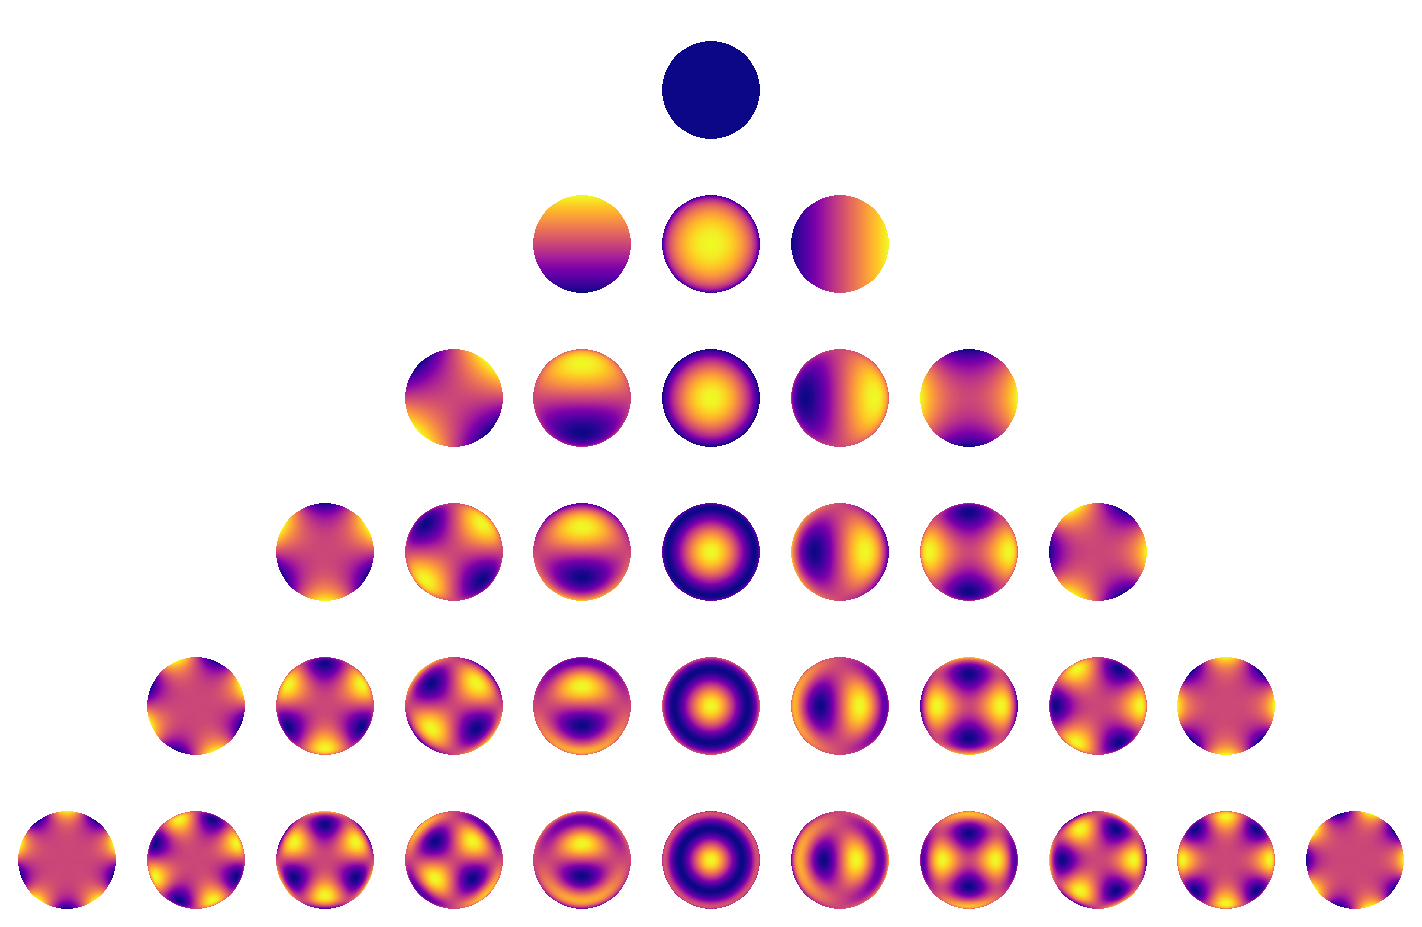
\includegraphics[width=\linewidth]{figures/ylms.pdf}
    \caption{\label{fig:ylms}
             \script{ylms}
             The real spherical harmonics up to order $l = 5$ computed from
             Equation~(\ref{eq:ylmxy}). In these plots, the $x$-axis points
             to the right, the $y$-axis points up, and the $z$-axis points
             out of the page. An animated version can be viewed
             \href{https://raw.githubusercontent.com/rodluger/%
                   cartograpy/gif/ylms.gif}{here}.}
    \end{centering}
\end{figure}
%
Since we are confined to the surface of the unit sphere, we have
$\z = \sqrt{1 - \x^2 - \y^2}$ and we may expand $\z^k$ using
the binomial theorem:
%
\begin{align}
    \z^{k} &= (1 - \x^2 - \y^2)^\frac{k}{2} \nonumber \\[0.5em]
          &=
          \begin{dcases}
              \sum_{p\,\mathrm{even}}^{k}
              \sum_{q\,\mathrm{even}}^p
              (-1)^\frac{p}{2}
              C_{pq}^{k}
              \x^{p-q} \y^{q}
              \qquad & k\,\mathrm{even} \\
              %
              \sum_{p\,\mathrm{even}}^{k - 1}
              \sum_{q\,\mathrm{even}}^p
              (-1)^\frac{p}{2}
              C_{pq}^{k-1}
              \x^{p-q} \y^{q} \sqrt{1 - \x^2 - \y^2}
              \qquad & k\,\mathrm{odd} \quad,
          \end{dcases}
          \label{eq:zk}
\end{align}
%
where
%
\begin{align}
    \label{eq:ckpq}
    C_{pq}^{k} =
    \frac{\left(\frac{k}{2}\right)!}{\left(\frac{q}{2}\right)!
    \left(\frac{k-p}{2}\right)! \left(\frac{p-q}{2}\right)!} \quad.
\end{align}
%
This gives us an expression for the spherical harmonic $Y_{lm}$
as a function of $\x$ and $\y$ only:
%
\begin{align}
    \label{eq:ylmxy}
    Y_{lm}(\x, \y) &=
    \begin{dcases}
        \!\begin{aligned}%[b]
            &
                \sum_{j\, \mathrm{even}}^m
                \sum_{k\, \mathrm{even}}^{l-m}
                \sum_{p\,\mathrm{even}}^{k}
                \sum_{q\,\mathrm{even}}^p
                \left(-1\right)^{\frac{j+p}{2}}
                A_{lm}
                B_{lm}^{jk}
                C_{pq}^{k}
                \x^{m - j + p - q}
                \y^{j + q}
            \, + \\
            &
                \sum_{j\, \mathrm{even}}^m
                \sum_{k\, \mathrm{odd}}^{l-m}
                \sum_{p\,\mathrm{even}}^{k - 1}
                \sum_{q\,\mathrm{even}}^p
                \left(-1\right)^{\frac{j+p}{2}}
                A_{lm}
                B_{lm}^{jk}
                C_{pq}^{k - 1}
                \x^{m - j + p - q}
                \y^{j + q}
                \z
       \end{aligned}
       &
       \quad m \ge 0 \\
       %
       %
       \\
       %
       %
       \!\begin{aligned}%[b]
           &
               \sum_{j\, \mathrm{odd}}^{|m|}
               \sum_{k\, \mathrm{even}}^{l-|m|}
               \sum_{p\,\mathrm{even}}^{k}
               \sum_{q\,\mathrm{even}}^p
               \left(-1\right)^{\frac{j+p-1}{2}}
               A_{l|m|}
               B_{l|m|}^{jk}
               C_{pq}^{k}
               \x^{|m| - j + p - q}
               \y^{j + q}
           \, + \\
           &
               \sum_{j\, \mathrm{odd}}^{|m|}
               \sum_{k\, \mathrm{odd}}^{l-|m|}
               \sum_{p\,\mathrm{even}}^{k - 1}
               \sum_{q\,\mathrm{even}}^p
               \left(-1\right)^{\frac{j+p-1}{2}}
               A_{l|m|}
               B_{l|m|}^{jk}
               C_{pq}^{k - 1}
               \x^{|m| - j + p - q}
               \y^{j + q}
               \z
      \end{aligned}
      &
      \quad m < 0
   \end{dcases}
    %
\end{align}
%
where $\z = \z(\x, \y) = \sqrt{1 - \x^2 - \y^2}$.



% ==============================================================================
% ------------------------------------------------------------------------------
% ------------------------------------------------------------------------------
\pagebreak
\section{Occultation Light Curves}
\label{sec:occultations}
% ------------------------------------------------------------------------------
% ------------------------------------------------------------------------------
% ==============================================================================

Consider a body of unit radius centered at the origin, with a surface map
given by the function $M(\x, \y)$,
being occulted by a body of radius $r$ centered at the point $(x_0, y_0)$.
The total flux radiated
in the direction of the observer is obtained by integrating the surface
map over the visible portion of the occulted body's disk:
%
\begin{align}
    \label{eq:occint}
    F &=
    \oiint M (\x, \y) \, \dd \bvec{A}
    = \int_{x_1}^{x_2}
      \int_{y_1}^{y_2}
      M (\x, \y) \, \dd \y \, \dd \x
      \quad,
\end{align}
%
where $x_1$ and $x_2$ are functions of $r$, $x_0$, and $y_0$, while
$y_1$ and $y_2$ are functions of $r$, $x_0$, $y_0$, and $\x$.
In general, this integral is
difficult (and often impossible) to compute directly.


%
%
\begin{figure}[p!]
    \begin{centering}
    \includegraphics[width=\linewidth]{figures/geometry.pdf}
    \caption{\label{fig:geometry}
             \script{geometry}
             Geometry of the occultation problem.
             The occulted body is centered
             at the origin and has unit radius, while the occultor
             is centered at $(x_0, y_0)$ and has radius $r$. We first rotate
             the two bodies about the origin through an angle
             $\theta = \nicefrac{\pi}{2} - \mathrm{arctan2}(y_0, x_0)$
             so the problem is symmetric about the $y$-axis. In this frame,
             the occultor is located at $(0, b)$, where
             $b = \sqrt{x_0^2 + y_0^2}$ is the impact parameter.
             The arc of the occultor
             that overlaps the occulted body (thick red curve) now extends from
             $\pi - \phi$ to $2\pi + \phi$, measured from the center of the
             occultor.
             The arc of the occulted body that is visible during
             the occultation (thick black curve) extends from
             $\pi - \lambda$ to $2\pi + \lambda$, measured from the origin.
             These are the curves along which the primitive integral
             (Equation~\ref{eq:primitive}) is evaluated.
             The angles $\phi$ and $\lambda$ are given by
             Equation~(\ref{eq:sinphi})
             and extend from $-\nicefrac{\pi}{2}$ to $\nicefrac{\pi}{2}$. When
             the occultor is completely within the disk of the occulted body,
             we define $\phi = \lambda = \nicefrac{\pi}{2}$.
             }
    \end{centering}
\end{figure}
%
%


One way to simplify the problem is to perform a
rotation through an angle $\theta = \nicefrac{\pi}{2} - \mathrm{arctan2}(y, x)$
about the $z$-axis so that the occultor lies along the $+y$-axis,
with its center located a distance $b = \sqrt{x_0^2 + y_0^2}$ from the origin
(see Figure~\ref{fig:geometry}).

\citet{MandelAgol2002}

\bibliography{starry}

\end{document}
